\documentclass[11pt,a4paper]{article}

\usepackage[T1]{fontenc}
\usepackage[utf8]{inputenc}
\usepackage{lmodern}
\usepackage{microtype}
\usepackage[a4paper,margin=2.5cm]{geometry}
\usepackage{graphicx}
\usepackage[table]{xcolor}
\usepackage{booktabs}
\usepackage{tabularx}
\usepackage{enumitem}
\usepackage{caption}
\usepackage{titlesec}
\usepackage{fancyhdr}
\usepackage{setspace}
\usepackage{float}
\usepackage{framed}
\usepackage[hidelinks]{hyperref}

\definecolor{navy}{HTML}{12263A}
\definecolor{teal}{HTML}{0F8B8D}
\definecolor{orange}{HTML}{E4572E}
\definecolor{lightgrey}{HTML}{EEF3F6}
\definecolor{midgrey}{HTML}{6B7785}

\hypersetup{colorlinks=true,linkcolor=navy,citecolor=teal,urlcolor=teal}
\setstretch{1.12}
\setlength{\parskip}{0.55em}
\setlength{\parindent}{0pt}
\setlist{itemsep=0.2em,topsep=0.3em}
\captionsetup{font=small,labelfont={bf,color=navy},labelsep=period,justification=raggedright,singlelinecheck=false}
\graphicspath{{figures/}}

\titleformat{\section}{\Large\bfseries\color{navy}}{\thesection}{0.7em}{}
\titleformat{\subsection}{\large\bfseries\color{navy}}{\thesubsection}{0.6em}{}
\titleformat{\subsubsection}{\normalsize\bfseries\color{teal}}{\thesubsubsection}{0.5em}{}
\titlespacing*{\section}{0pt}{1.6em}{0.5em}
\titlespacing*{\subsection}{0pt}{1.1em}{0.3em}

\pagestyle{fancy}
\fancyhf{}
\renewcommand{\headrulewidth}{0.3pt}
\fancyhead[L]{\small\color{midgrey}Medical VQA for Chest X-rays}
\fancyhead[R]{\small\color{midgrey}Project Report}
\fancyfoot[C]{\small\thepage}

\newcommand{\placeholder}[1]{\textcolor{orange}{[#1]}}
\colorlet{shadecolor}{lightgrey}
\newenvironment{keybox}{\begin{shaded}\small}{\end{shaded}}

\begin{document}

% ------------------------------------------------------------------ title page
\begin{titlepage}
\thispagestyle{empty}
\vspace*{1.2cm}
{\color{teal}\rule{3.2cm}{3pt}}\par\vspace{0.8cm}
{\sffamily\bfseries\fontsize{26}{32}\selectfont\color{navy} Medical Visual Question Answering for Chest X-rays\par}
\vspace{0.5cm}
{\sffamily\large\color{midgrey} A knowledge-grounded approach with CheXagent-2-3b:\\ literature review, baseline tests and retrieval-augmented design\par}
\vspace{1.0cm}
{\sffamily\bfseries\large\color{navy} PROJECT REPORT\par}
\vspace{2.2cm}

\begin{tabular}{@{}p{4.2cm}p{9cm}@{}}
\textbf{Supervisor} & \placeholder{Supervisor name, designation} \\[1.1em]
\textbf{Submitted by} & \placeholder{Team member 1, roll number} \\
 & \placeholder{Team member 2, roll number} \\
 & \placeholder{Team member 3, roll number} \\[1.1em]
\textbf{Department} & \placeholder{Department / programme} \\[1.1em]
\textbf{Institution} & \placeholder{Institution name} \\[1.1em]
\textbf{Date} & \placeholder{Month Year} \\
\end{tabular}

\vfill
{\small\color{midgrey} Names, institution and date are placeholders and will be replaced with the official title-page format.\par}
\end{titlepage}

% ------------------------------------------------------------------ abstract
\pagenumbering{roman}
\section*{Abstract}
Visual question answering (VQA) lets a person ask a free-text question about a medical image and receive a free-text answer.
This project studies VQA on chest X-rays with a small open model, \textsc{CheXagent-2-3b}, that runs on a free Colab T4 GPU.
We reviewed six papers, kept three that shaped the plan (CheXagent, RULE, Med-Flamingo), and built a pre-registered
evaluation: the rules, test sets and success conditions were written down before any model run.
Zero-shot tests on 219 baseline questions, 130 knowledge questions, 140 left/right questions and a set of mirror-image
pairs gave an overall accuracy of 58\%, with weak left/right and knowledge scores.
Disease naming on 130 images then produced the same answer for every image, which led us to the central finding of the
work so far: \textbf{in every run to date the image never reached the model}, because of a software-version
incompatibility. The earlier numbers are therefore a text-only control, not a measurement of the model's perception.
We fixed the problem, added an automatic image check to every notebook, and corrected all earlier documents.
In parallel we designed a knowledge-grounded retrieval pipeline (name the disease, then retrieve from MedlinePlus and medical
textbooks) and measured, without any model, how often the corpus holds the gold answer: 29\% of gold items on held-out
questions with the true disease, 17\% with a wrong disease and 3\% from the question alone.
No result with the image visible exists yet; those runs are the next step. The work makes no clinical-validity claim.

\tableofcontents
\clearpage
\listoffigures
\clearpage
\pagenumbering{arabic}

% ------------------------------------------------------------------ 1 introduction
\section{Introduction}
\subsection{Motivation}
Chest X-rays are among the most common medical images, and reading them takes training.
A system that can answer plain questions about an X-ray (``Is the heart enlarged?'', ``Which side is the fluid on?'',
``What causes this disease?'') could one day support teaching and report drafting.
Recent vision-language models can produce such answers, but how reliable they are, and why, is not well understood.
This project is a careful, small-scale investigation of that question, not a clinical tool.

\subsection{Objectives}
\begin{enumerate}
\item Explain what chest X-rays show and what medical VQA asks of a model.
\item Review the literature and keep only the findings that change what we do.
\item Measure how a ready-made chest X-ray model, \textsc{CheXagent-2-3b}, answers questions without any extra training.
\item Design and test a knowledge-grounded retrieval extension, and decide beforehand how success will be judged.
\item Report honestly, including results that went against our expectations.
\end{enumerate}

\subsection{Scope and standards}
The project follows four standards from the start: plain-language explanations, strict honesty about limits, no claim of
clinical validity, and pre-registration (rules fixed before running the model). Everything described here is reproducible
from the project repository; Section~\ref{sec:repro} lists the main files.

% ------------------------------------------------------------------ 2 background
\section{Background}
\subsection{What a chest X-ray shows}
A chest X-ray is a shadow picture. X-rays pass easily through air and are stopped by dense tissue, so air-filled lungs
appear dark and bone, fluid and the heart appear white. The standard frontal view is the posterior-anterior (PA) film.
By convention the patient's right appears on the left of the image, which matters later for left/right questions.

\begin{figure}[H]
\centering
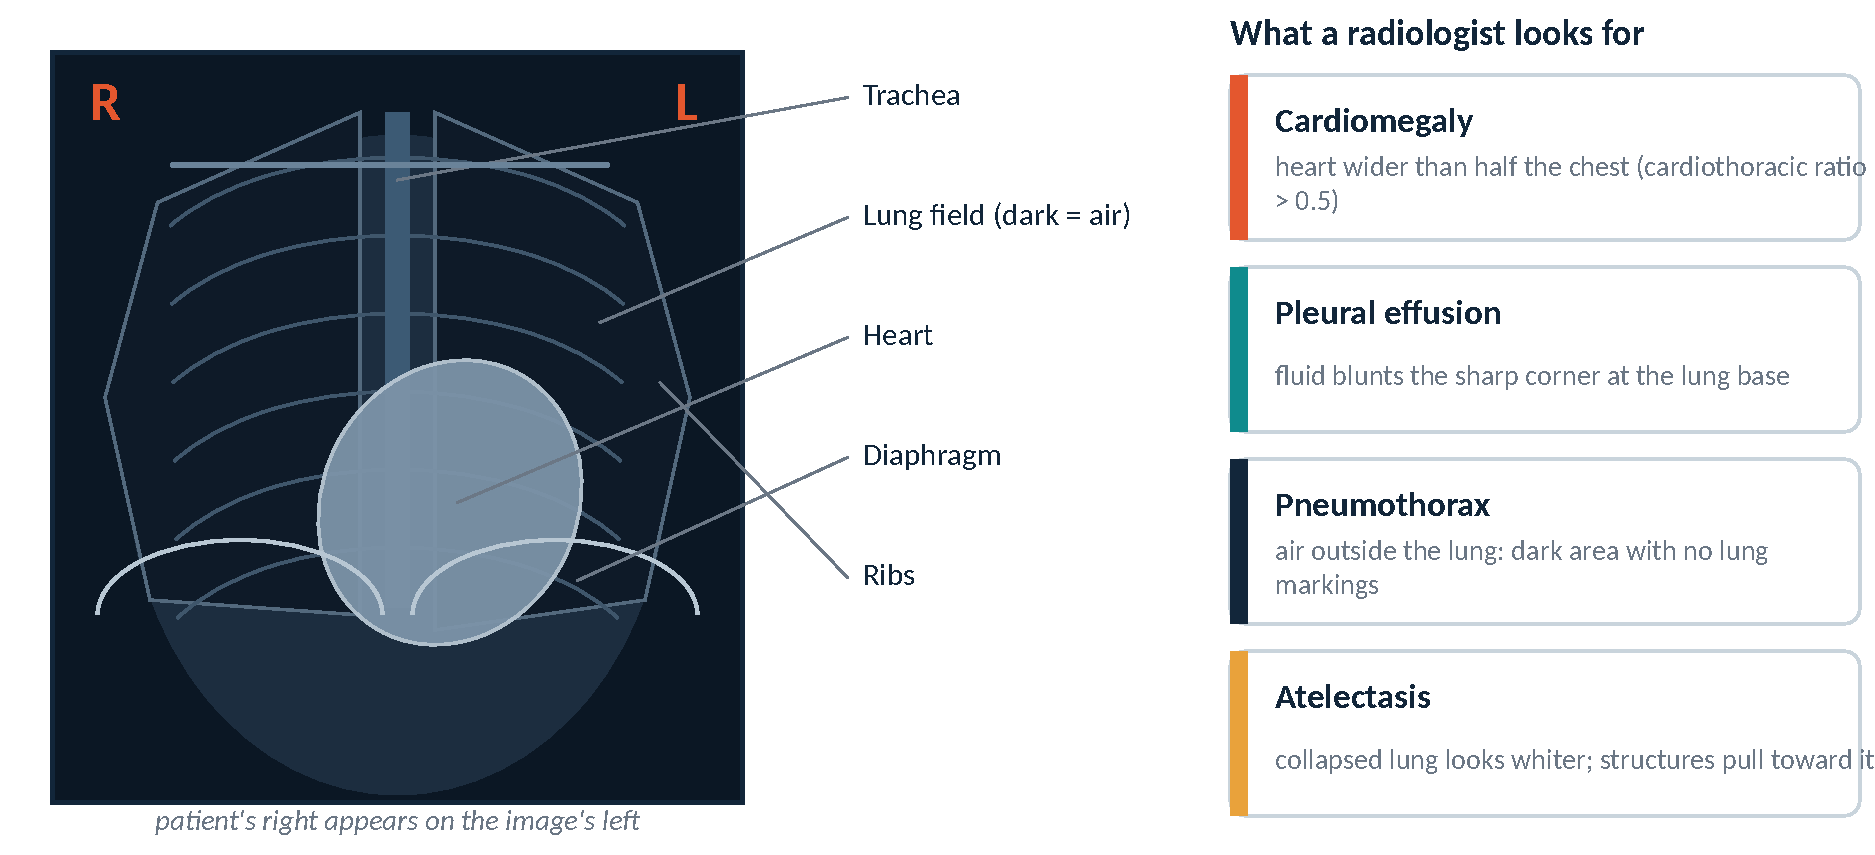
\includegraphics[width=\linewidth]{fig_cxr_anatomy.pdf}
\caption{Schematic of a frontal chest X-ray (drawn for this report, not a real image) and four findings that occur often in
the question sets used here.}
\label{fig:anatomy}
\end{figure}

Four findings recur throughout the project (Figure~\ref{fig:anatomy}):
\begin{itemize}
\item \textbf{Cardiomegaly}: an enlarged heart, usually judged by a cardiothoracic ratio above 0.5 (heart width over chest width).
\item \textbf{Pleural effusion}: fluid around the lung, which blunts the sharp angle where the diaphragm meets the chest wall.
\item \textbf{Pneumothorax}: air outside the lung, seen as a dark area with no lung markings and a visible pleural line.
\item \textbf{Atelectasis}: partly collapsed lung, which looks whiter and pulls nearby structures toward it.
\end{itemize}

\subsection{Medical visual question answering}
In medical VQA the model receives an image and a question and must write an answer (Figure~\ref{fig:vqa}).
We separate two kinds of difficulty, because they fail in different ways:
\textbf{perception} (seeing the finding in the picture) and \textbf{knowledge} (knowing facts about the disease, such as its
cause or treatment).

\begin{figure}[H]
\centering
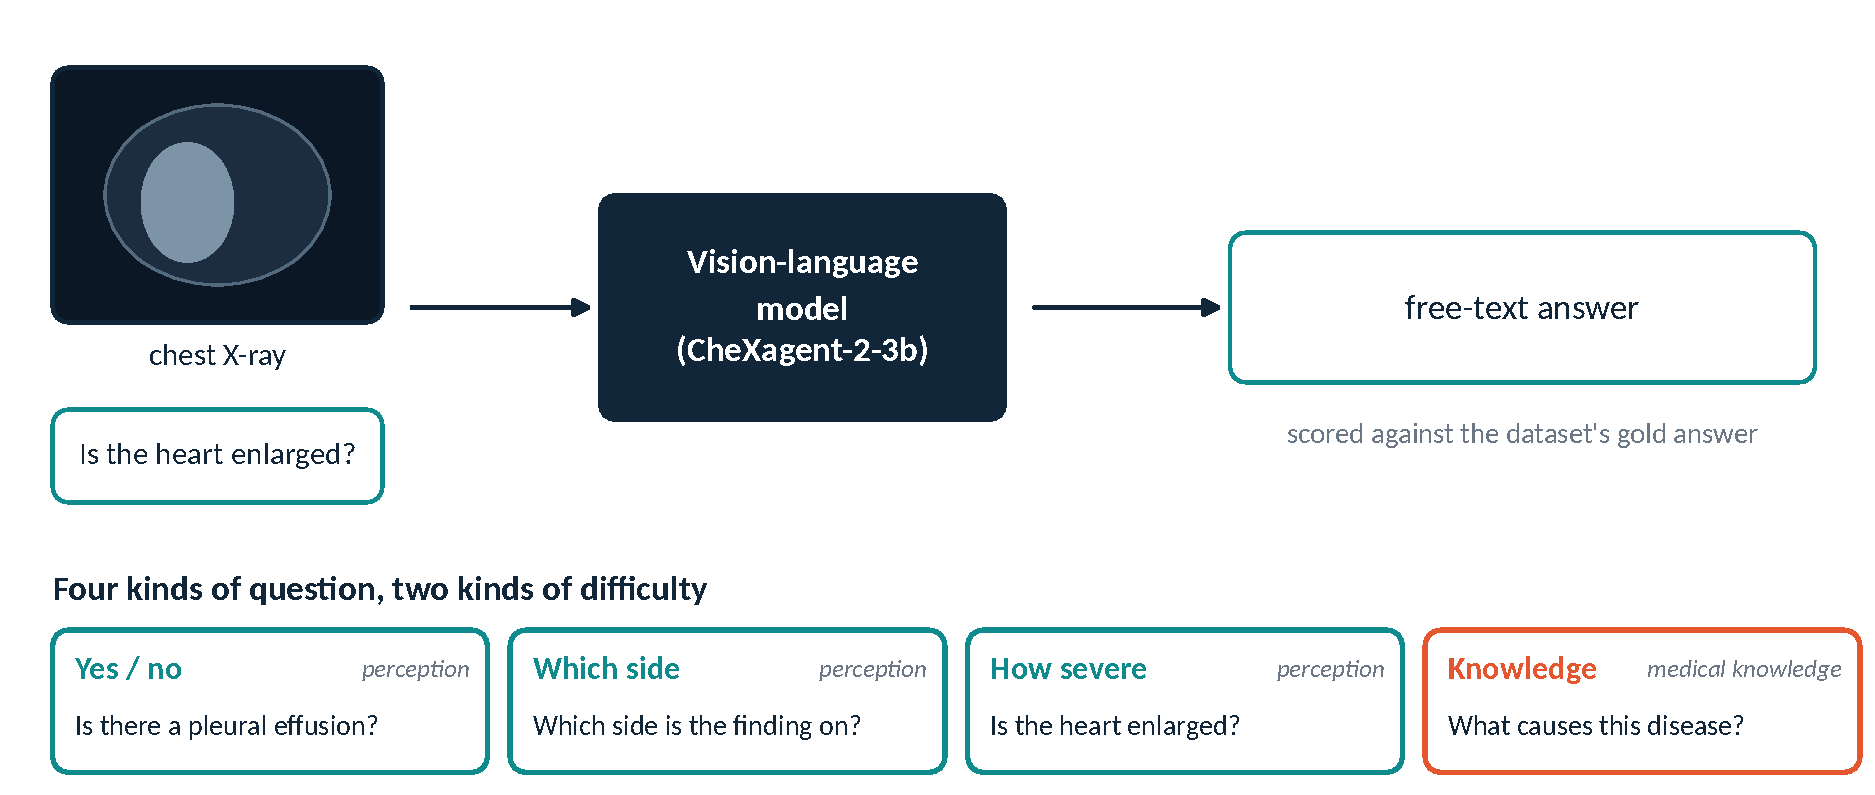
\includegraphics[width=\linewidth]{fig_vqa_task.pdf}
\caption{The task. Yes/no, side and severity questions test perception; knowledge questions test what the model knows about
a disease.}
\label{fig:vqa}
\end{figure}

\subsection{Datasets and model}
\textbf{SLAKE}~\cite{slake} and \textbf{VQA-RAD}~\cite{vqarad} are radiology VQA datasets with expert-written questions.
We use their chest X-ray questions only. SLAKE additionally gives each image a set of labels, which we turn into a
disease label for 130 chest images across eight classes (cardiomegaly 29, atelectasis 21, mass 19, nodule 18, pneumonia 17,
effusion 13, pneumothorax 10, infiltration 9).
The model is \textbf{CheXagent-2-3b}~\cite{chexagent}, a 3.1-billion-parameter vision-language model trained on chest X-ray
instruction data. Its training data (CheXinstruct) already includes SLAKE and VQA-RAD, so our tests are close to
in-distribution rather than a clean held-out test.

% ------------------------------------------------------------------ 3 literature
\section{Literature review}
We reviewed six papers and keep three here because they changed the plan; the other three gave useful context.

\subsection{Papers that shaped the project}
\textbf{CheXagent}~\cite{chexagent} is the only model in our review built end to end for chest X-rays. It was trained on
CheXinstruct, a collection of 8.5 million instruction triplets from 32 datasets covering 35 tasks, and outperforms larger
general-purpose medical models. Its own results show where it is weakest: fine-grained reasoning such as side and severity
reaches only 77--79\%, against over 90\% on coarse tasks. We chose it as the baseline model, and treat left/right and
heart-size questions as the hardest perception cases.

\textbf{RULE}~\cite{rule} adds retrieval to a medical vision-language model and shows why naive retrieval backfires.
Too few or too many retrieved passages hurt, and the model over-trusts retrieved text: among errors introduced by retrieval,
47.4\%, 47.4\% and 58.7\% (IU-Xray, FairVLMed, MIMIC-CXR) were cases where the model had answered correctly without it.
RULE retrieves similar case reports, not authoritative knowledge. For us this means: keep retrieved text short, check
that retrieval does no harm, and include an arm that supplies only the disease name without any retrieved text.

\textbf{Med-Flamingo}~\cite{medflamingo} evaluates answers with clinicians and finds that automatic scores can disagree with
clinical judgement. We therefore plan a blind 0/1/2 rating of answers and avoid relying on a single automatic score.

\subsection{Context papers}
\textbf{PubMedCLIP}~\cite{pubmedclip} found that the image encoder matters far more than the text encoder for medical VQA.
\textbf{LLaVA-Med}~\cite{llavamed} shows cheap curriculum tuning of a general model on GPT-4-written instruction data, which
carries a hallucination risk because the writer never saw the image.
\textbf{PMC-VQA}~\cite{pmcvqa} builds questions from figure captions, and even with filtering such questions can often be
answered from text alone, a warning that we later met directly (Section~\ref{sec:bug}).

\begin{figure}[H]
\centering
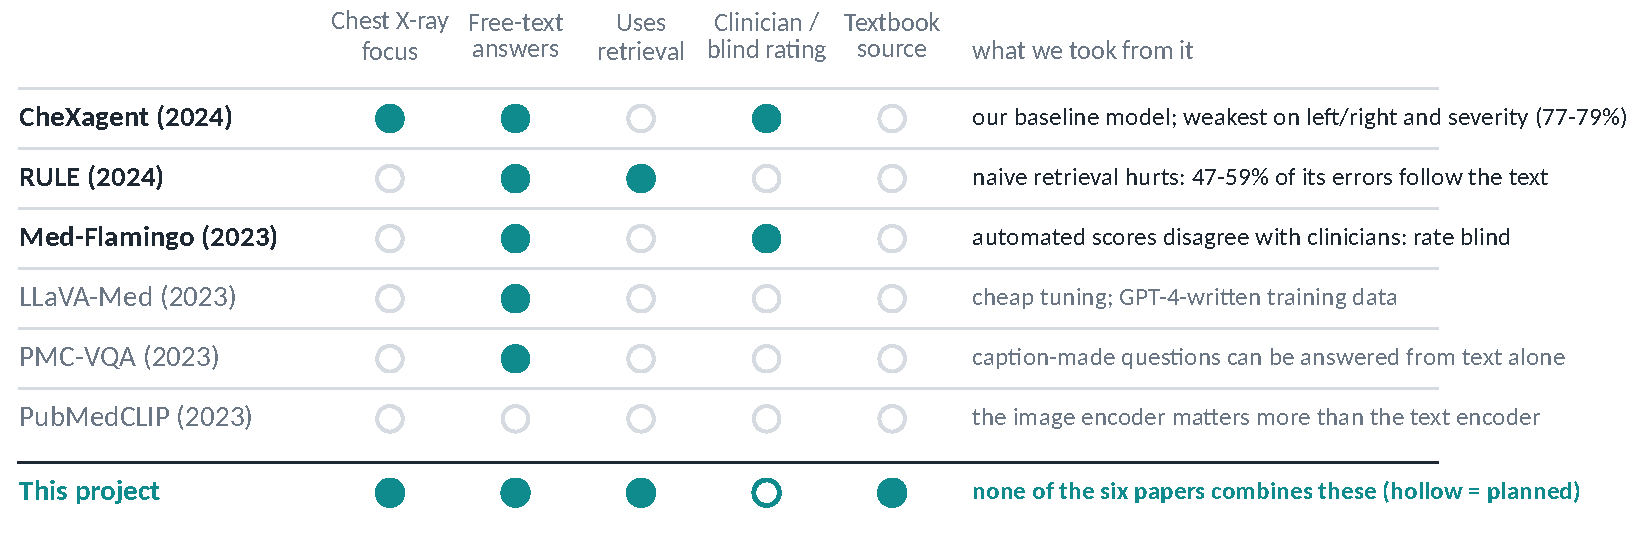
\includegraphics[width=\linewidth]{fig_papers_matrix.pdf}
\caption{Comparison of the six papers and this project. Highlighted rows shaped the plan; the hollow circle marks the blind
rating that is planned but not yet done.}
\label{fig:matrix}
\end{figure}

\subsection{Gap and design decisions}
Among the papers reviewed, none combines a chest-X-ray model with retrieval of authoritative knowledge and a careful,
pre-registered evaluation. Figure~\ref{fig:gaps} shows how each finding became a concrete decision.

\begin{figure}[H]
\centering
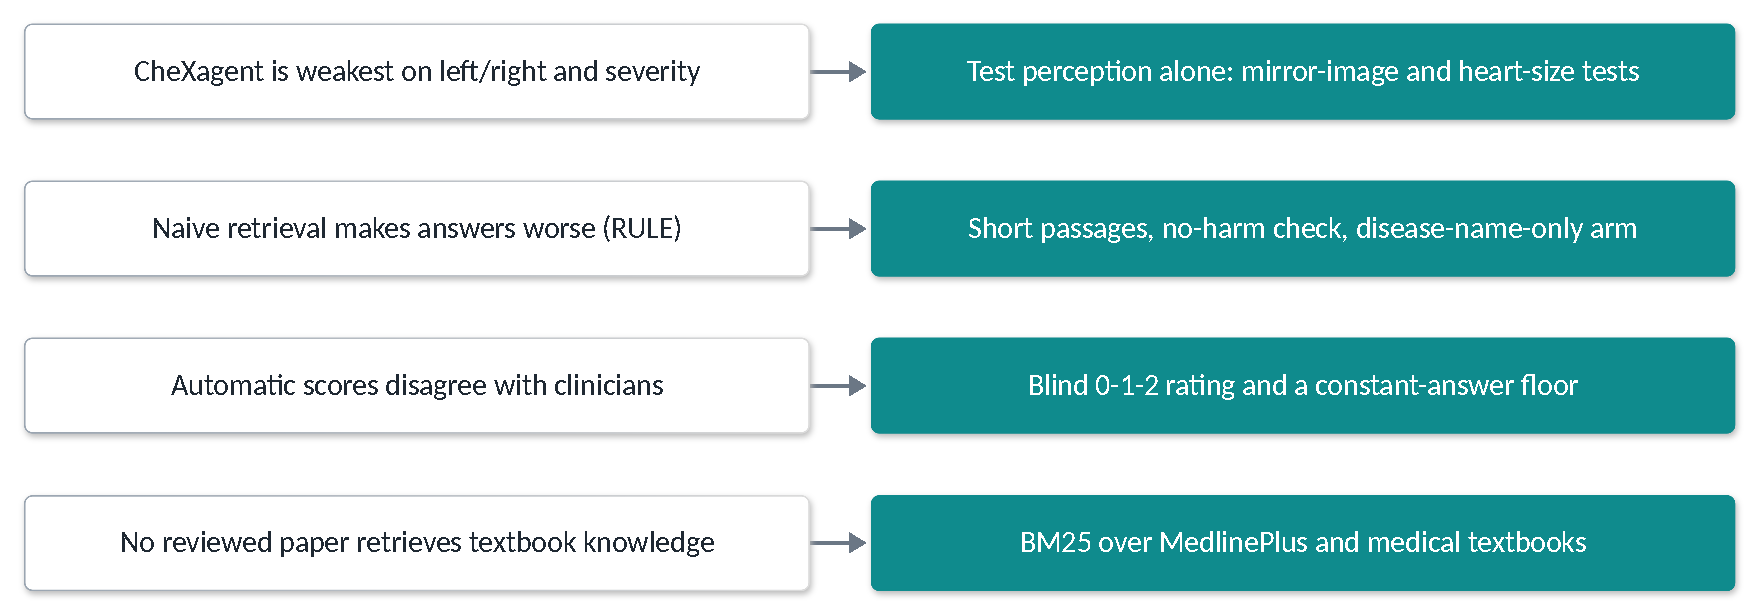
\includegraphics[width=\linewidth]{fig_gaps_to_plan.pdf}
\caption{From literature findings to design decisions.}
\label{fig:gaps}
\end{figure}

% ------------------------------------------------------------------ 4 methodology
\section{Evaluation method}
\subsection{Pre-registration}
Before any run we wrote the rules into \texttt{docs/evaluation\_protocol.md}: the test sets, the scorer, the statistics
and the conditions that would count as success. Changes are recorded as dated amendments (six so far) rather than silent
edits. Figure~\ref{fig:protocol} shows the flow.

\begin{figure}[H]
\centering
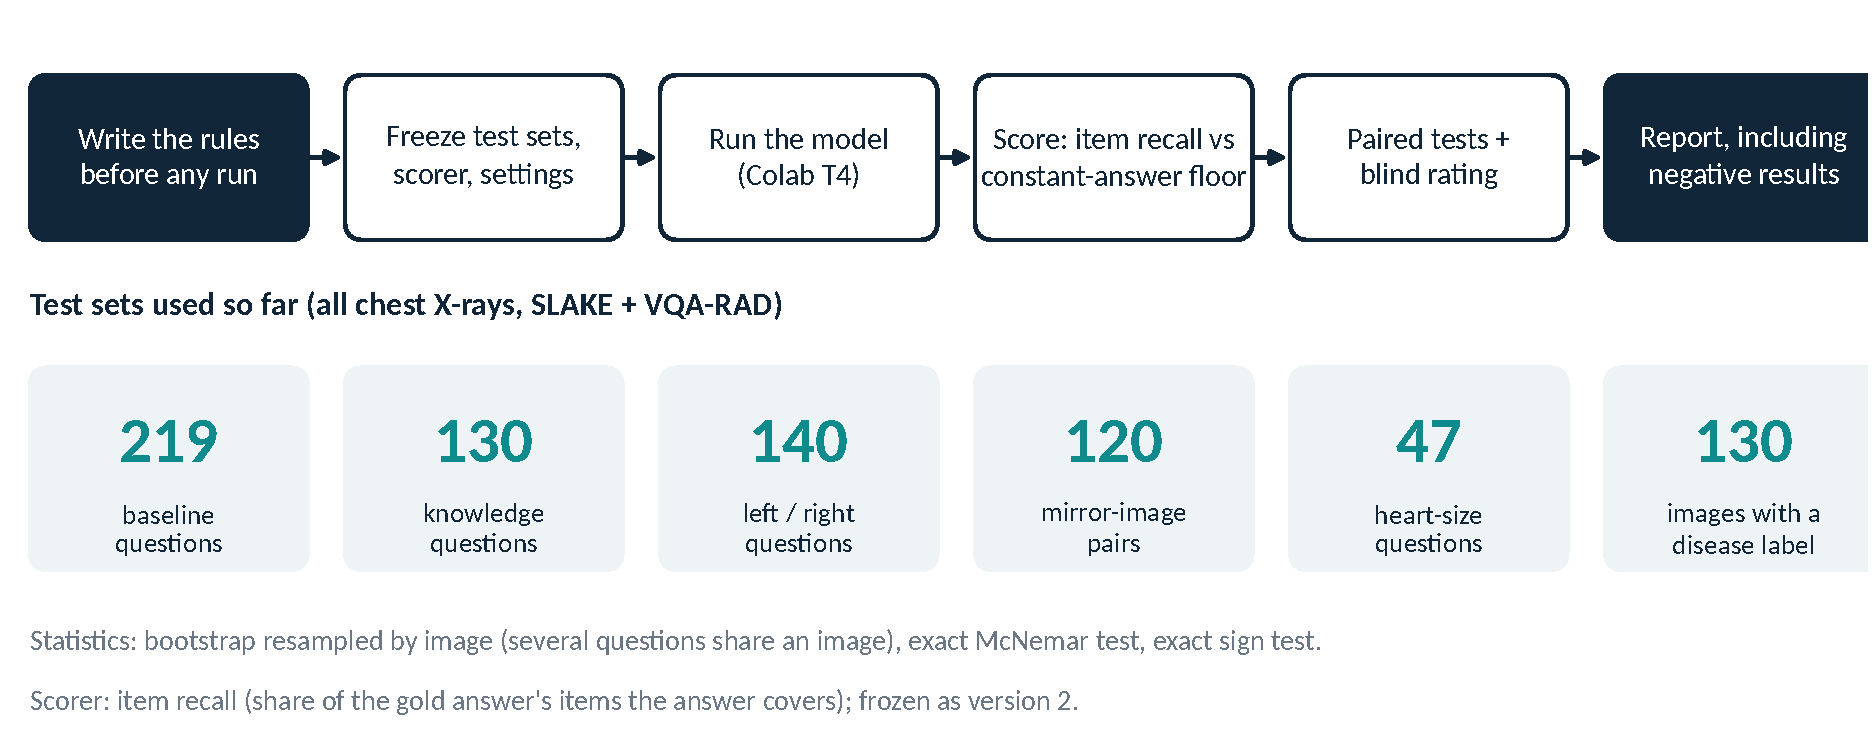
\includegraphics[width=\linewidth]{fig_eval_protocol.pdf}
\caption{Evaluation flow and the test sets used so far.}
\label{fig:protocol}
\end{figure}

\subsection{Scoring}
\begin{itemize}
\item \textbf{Exact match and loose match} for short answers (yes/no, one word).
\item \textbf{Item recall} for list-style answers: the share of the gold answer's items that the model's answer covers
(scorer version~2, frozen).
\item \textbf{Constant-answer floor}: the score of a system that ignores the image and always writes the most common gold
answer for that question type (leave-one-out). A real system must beat this floor.
\item \textbf{Statistics}: bootstrap resampled by image, because several questions share one image; exact McNemar test for
paired yes/no outcomes; exact sign test for paired scores.
\end{itemize}

\subsection{Test sets}
\begin{table}[H]
\centering
\small
\begin{tabular}{@{}lrl@{}}
\toprule
Set & Size & Purpose \\
\midrule
Pilot & 60 & First feasibility run \\
Baseline (run 2) & 219 & General, left/right and severity questions \\
Knowledge (run 3) & 130 & Symptoms, treatment, cause, prevention, function, why \\
Side (run 3) & 140 & Questions whose answer is a side \\
Mirror pairs (run 4) & 120 & Same question on an image and its mirror \\
Heart-size (run 4) & 47 & ``Is the heart enlarged?'' wordings \\
Disease labels (run 5) & 130 & Naming the disease from the image \\
\bottomrule
\end{tabular}
\caption{Test sets. Five questions were removed from the original 224-question baseline after a keyword-filter bug
admitted non-chest images (Section~\ref{sec:baseline}).}
\label{tab:sets}
\end{table}

% ------------------------------------------------------------------ 5 results
\section{Experiments and results to date}
\begin{figure}[H]
\centering
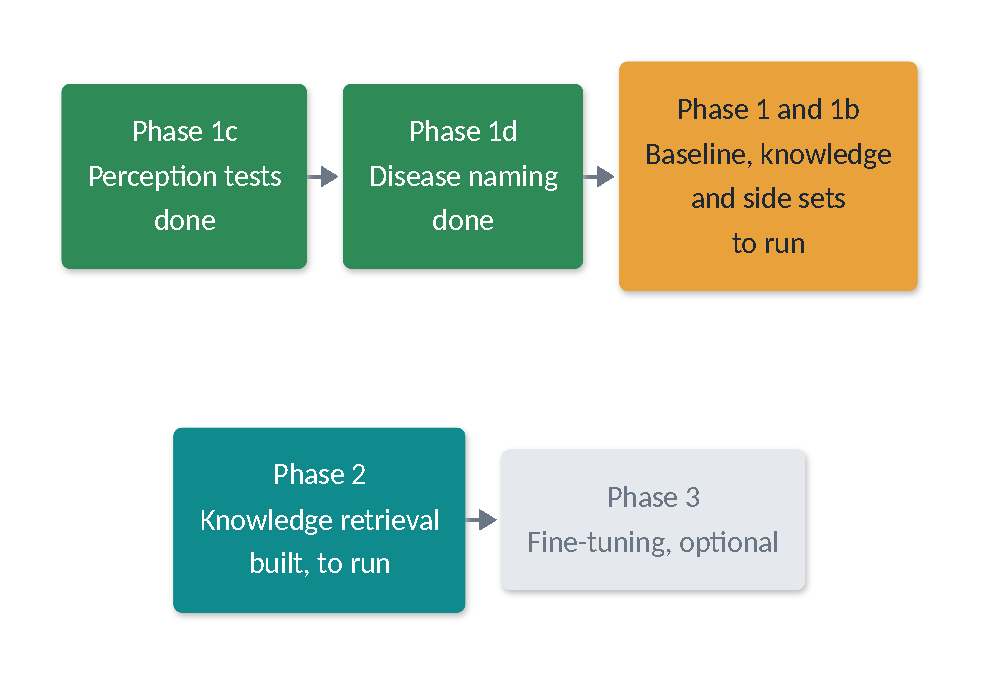
\includegraphics[width=\linewidth]{fig_roadmap.pdf}
\caption{Project phases and their status. The asterisk marks runs in which the image did not reach the model.}
\label{fig:roadmap}
\end{figure}

\begin{keybox}
\textbf{Important reading note.} Sections~\ref{sec:baseline} to~\ref{sec:diag} report runs in which the model answered from
the question text alone (see Section~\ref{sec:bug}). They are valid as a \emph{text-only control}: they show how much of
these benchmarks can be solved without the image. They do \textbf{not} show what the model can or cannot read from an
X-ray. Conclusions about perception are withdrawn until the runs are repeated with the fix.
\end{keybox}

\subsection{Zero-shot baseline}\label{sec:baseline}
The first pilot on 60 questions scored 37 of 60 (61.7\%). The larger run (219 questions after removing five rows that were
probably not chest images) is summarised in Table~\ref{tab:baseline}.

\begin{table}[H]
\centering
\small
\begin{tabular}{@{}lrrr@{}}
\toprule
Question type & Correct / total & Accuracy & 95\% interval \\
\midrule
Overall & 128 / 219 & 58.4\% & 52--65\% \\
General & 70 / 96 & 72.9\% & 63--81\% \\
Left/right & 44 / 100 & 44.0\% & 35--54\% \\
Severity & 14 / 23 & 60.9\% & 41--78\% \\
\bottomrule
\end{tabular}
\caption{Run 2 (text-only control). Intervals are Wilson 95\%.}
\label{tab:baseline}
\end{table}

On the 22 heart-size yes/no questions the model answered ``no'' every time, although the gold answer was ``yes'' in eight.
Left/right accuracy was lower than general accuracy, but the comparison is partly confounded by dataset and question
style, so we treat it as likely rather than settled.

\subsection{Knowledge questions}
On 105 knowledge questions (excluding 25 ``function'' questions whose gold answer is always ``Breathe'') the model reached
an item recall of 0.37, against 0.38 for the constant-answer floor (Figure~\ref{fig:textonly}, middle).
It was above the floor only on symptoms (0.42 against 0.21), matched it on treatment and cause, and fell below it on
prevention, where it wrote ``keeping healthy'' while the gold answers were mostly different phrasings.
The 130 knowledge questions have only 33 distinct gold answers, so the answer is largely determined by which disease is in the
image; this observation motivates the two-step design in Section~\ref{sec:phase2}.

\subsection{Perception diagnostics}\label{sec:diag}
Two diagnostics were run on left/right behaviour.
In the \textbf{mirror test}, each question was asked on the original image and on its horizontal mirror. A model that reads
laterality should swap its answer. Of 73 pairs in which a side was named on both images, only 2 swapped (3\%), and
112 of 120 answers were byte-identical; on the 29 explicit ``which side'' questions, 29 of 29 were identical and 26 of 29
answers were ``Right''.
In the \textbf{wording test}, six prompt wordings were tried on 60 side questions; none fixed the behaviour.
A heart-size wording test found a weak signal (sensitivity 9 of 22, specificity 22 of 25) below the bar fixed in advance.

\begin{figure}[H]
\centering
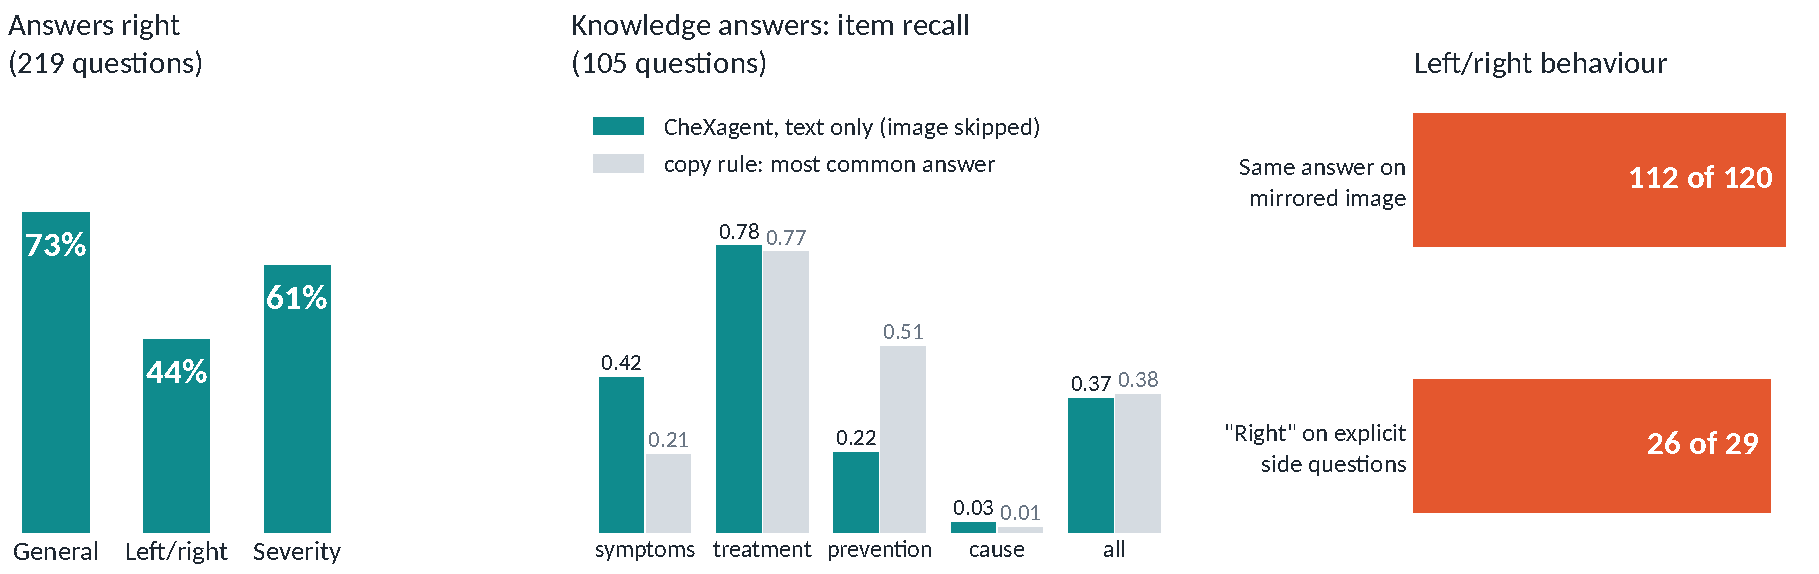
\includegraphics[width=\linewidth]{fig_text_only_results.pdf}
\caption{Text-only control results. Left: accuracy by question type with 95\% intervals (219 questions). Middle: knowledge
item recall against the constant-answer floor (105 questions). Right: left/right behaviour (mirror test).}
\label{fig:textonly}
\end{figure}

\subsection{Disease naming and the turning point}\label{sec:bug}
Phase~1d asked the model to name the disease on 130 labelled images in three ways (open question, forced choice,
one-versus-rest scoring per class). All 130 images received the same answer under each method, per-class scores varied by
only 0.002--0.009, and accuracy was 13\% (open), 0\% (forced) and 7\% (per-class), against a majority-class rate of 22\%.
Identical answers on every image are not a perception failure; they are what one would expect if the model could not see the image.

\textbf{Cause.} With \texttt{transformers} 4.46.3 the generation routine passes an \emph{empty} cache object to the model.
CheXagent's own code encodes the image only when that cache is \texttt{None}, so the image branch was skipped silently
and every answer came from the text of the prompt alone (Figure~\ref{fig:bug}).

\textbf{Fix and safeguard.} We patched the condition so that an empty cache still encodes the image, and added an
\textbf{IMAGE CHECK} to every notebook: the same file path is used with black, white and noise pixels, and the run stops
if the output log-probabilities do not change by at least 0.01.

\textbf{Consequences.} All earlier documents now carry a correction banner (Amendment~6 of the protocol, experiment log
entry~17). The earlier runs remain useful as a text-only control: 58\% overall accuracy, with no image at all, shows how
much of these benchmarks can be answered from the question wording alone, which is the same shortcut risk that
PMC-VQA warns about. Conclusions about left/right and heart-size perception are withdrawn until the reruns
(notebooks 04 and 05, then 01--03).

\begin{figure}[H]
\centering
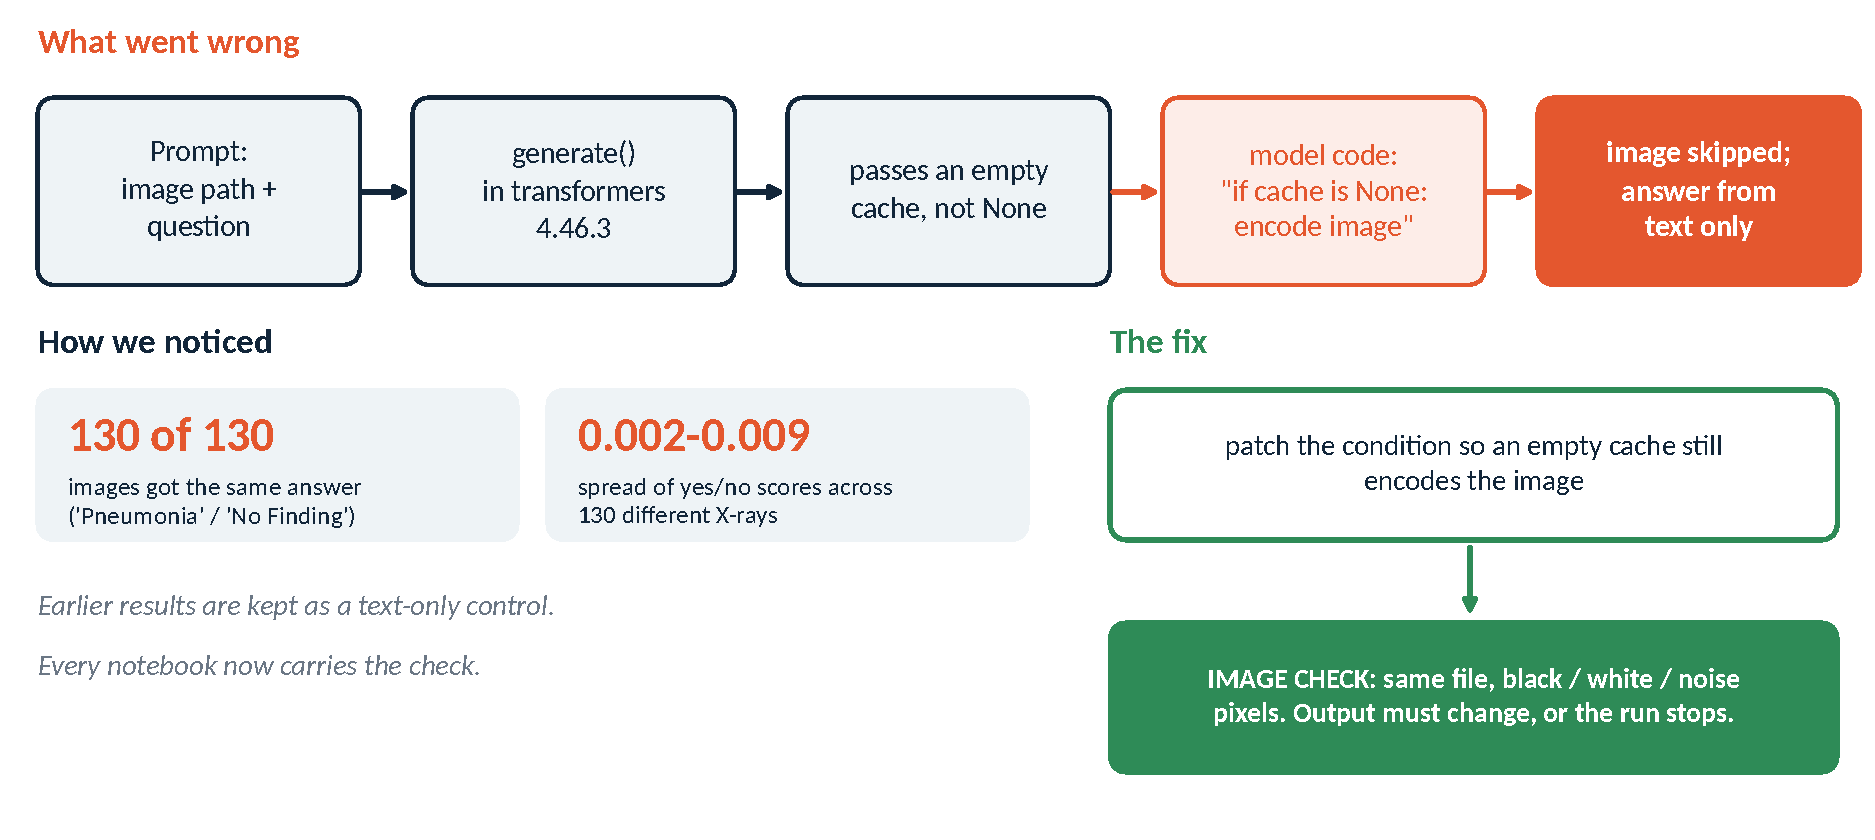
\includegraphics[width=\linewidth]{fig_bug_flow.pdf}
\caption{The image-skipping fault, how it was noticed, and the fix.}
\label{fig:bug}
\end{figure}

% ------------------------------------------------------------------ 6 phase 2
\section{Phase 2: knowledge-grounded retrieval}\label{sec:phase2}
\subsection{Design}
SLAKE's knowledge questions never name the disease (``What symptoms will the disease on the left bring?''), and the gold
answer is effectively a lookup keyed by the disease on the image. The system therefore works in two steps
(Figure~\ref{fig:pipeline}): (a)~name the disease from the image, a perception step; (b)~retrieve what is known about that
disease and let the model answer with the passages in its prompt, a knowledge step.

Retrieval uses our own BM25 implementation over two corpora that are independent of the test data: \textbf{MedlinePlus}
(US National Library of Medicine, public domain) and the 18 medical textbooks of the MedRAG collection~\cite{medrag}.
The textbooks are copyrighted, so they are downloaded at run time into a git-ignored folder and never committed.
The retrieval setting (topic lookup plus textbooks, two passages, 700 characters each) was chosen on 16 development questions
only and frozen before held-out numbers were computed.

\begin{figure}[H]
\centering
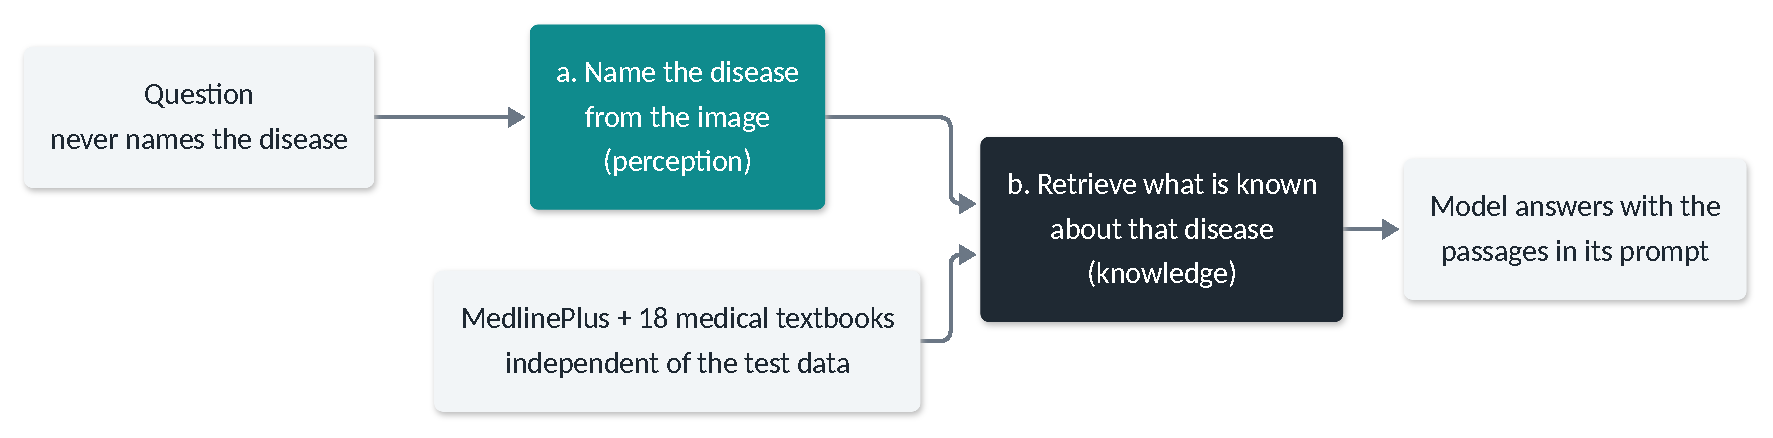
\includegraphics[width=\linewidth]{fig_rag_pipeline.pdf}
\caption{The two-step pipeline and the reason for it.}
\label{fig:pipeline}
\end{figure}

\subsection{Experimental arms}
Six arms (Figure~\ref{fig:arms}) separate the value of knowing the disease from the value of retrieval.
Oracle arms (A2--A4) use SLAKE's own disease label, which a real system would not have, so they are upper bounds and never
reported as the result. The real system is A6. Amendment~5 requires A6 to beat both the fair baseline A1 and the
guess-only arm A5, so a gain that comes only from naming the disease cannot be credited to retrieval.

\begin{figure}[H]
\centering
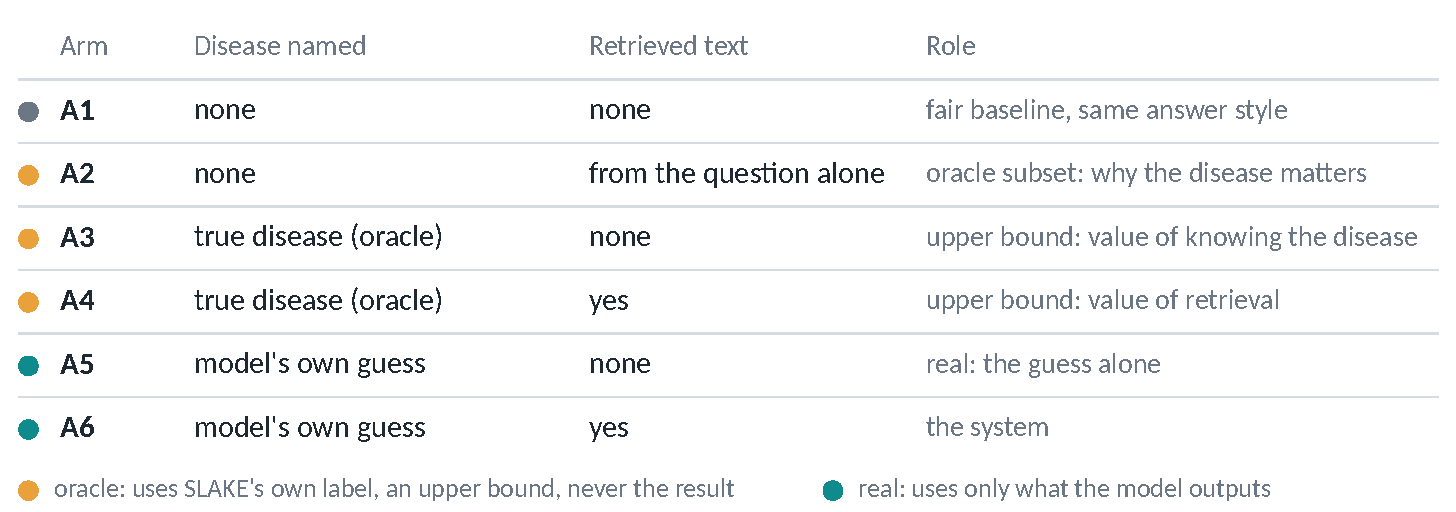
\includegraphics[width=\linewidth]{fig_arms.pdf}
\caption{The six experimental arms.}
\label{fig:arms}
\end{figure}

\subsection{Retrieval check without a model}
Before spending any GPU time we measured how often the retrieved text contains the gold answer's items (Table~\ref{tab:retrieval},
Figure~\ref{fig:retrieval}). ``Strict'' coverage requires the gold item's words to appear within one sentence.

\begin{table}[H]
\centering
\small
\begin{tabular}{@{}lrrr@{}}
\toprule
Retrieval query & Dev (n=16) & Held-out (n=34) & All 50 \\
\midrule
True disease & 0.42 & 0.29 & 0.33 \\
Wrong disease & 0.16 & 0.17 & 0.13 \\
Question only & 0.05 & 0.03 & 0.04 \\
\bottomrule
\end{tabular}
\caption{Strict gold-item coverage of the retrieved text. The setting was tuned on the development questions only.}
\label{tab:retrieval}
\end{table}

\begin{figure}[H]
\centering
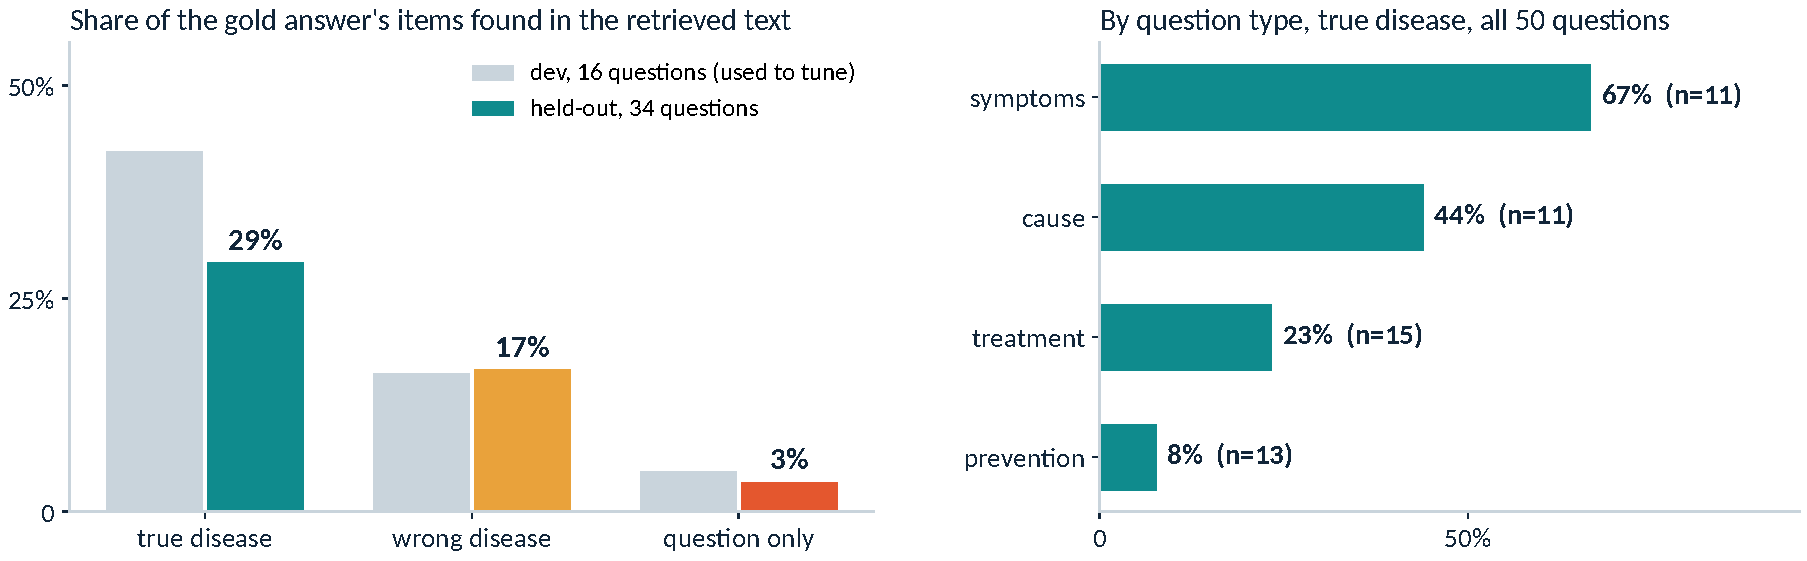
\includegraphics[width=\linewidth]{fig_retrieval_results.pdf}
\caption{Left: coverage by query type. Right: coverage by question type with the true disease (all 50 questions).}
\label{fig:retrieval}
\end{figure}

Three readings follow. First, the corpus holds more of the answer when the disease is right, and almost none when only the
question is used, which supports the two-step design. Second, coverage is an upper limit on what retrieval can add: even the
best case covers about a third of the gold items. Third, it differs by question type (symptoms 67\%, cause 44\%,
treatment 23\%, prevention 8\%), because generic gold phrases such as ``keep healthy'' almost never match a source sentence.
A router that sends only knowledge questions to retrieval (25 of 219 baseline questions routed, all in the knowledge set)
was also checked, to ensure retrieval cannot affect perception questions.

% ------------------------------------------------------------------ 7 status
\section{Status, limitations and next steps}
\subsection{Where the work stands}
Built and tested: the baseline pipeline, all test sets, the scorers and analysis scripts, the retrieval pipeline and corpora
loaders, the disease-naming and retrieval notebooks, and 121 automated tests (using stand-in models to check the plumbing).
Not yet done: any model run with the image visible.

\subsection{Next steps}
\begin{enumerate}
\item Rerun the disease-naming notebook (04) first with the IMAGE CHECK, then in full, to see whether the model can name the
disease at all when it sees the image. This sets the ceiling for the whole retrieval system.
\item Run the retrieval notebook (05) with the disease method chosen in step~1.
\item Rerun notebooks 01--03 to replace the text-only control with real perception measurements.
\item Collect blind 0/1/2 ratings of a sample of answers.
\item Consider targeted fine-tuning (Phase~3) only if Phase~2 shows a gap worth closing.
\end{enumerate}

\subsection{Limitations}
\begin{itemize}
\item Zero-shot only, one model, and small test sets (the retrieval check has 50 questions).
\item SLAKE's knowledge answers are annotator-written templates, so a high score does not imply clinical knowledge.
\item CheXagent's training data includes SLAKE and VQA-RAD, so the tests are not a clean held-out evaluation.
\item The disease labels come from SLAKE annotations and cover eight classes only.
\item No clinician has reviewed any output. Nothing in this report supports a claim of clinical validity or safety.
\end{itemize}

% ------------------------------------------------------------------ 8 conclusion
\section{Conclusion}
The literature review gave a clear, narrow question: can retrieved textbook knowledge improve a chest-X-ray model's answers
to knowledge questions, without making perception questions worse? We built an evaluation that fixes the rules in advance and
a retrieval pipeline that measurably contains the answer more often when the disease is known.
The most important result so far is a negative and instructive one: in every run, the image did not reach the model. Because of
the safeguards we had set up (a constant-answer floor, identical-answer checks, pre-registered readings), the fault was
found and traced to a software-version incompatibility, and the earlier numbers were relabelled as a text-only control instead
of being reported as perception results.
The next stage is a clean set of runs with the image visible, starting with disease naming.

% ------------------------------------------------------------------ references
\begin{thebibliography}{99}\small
\setlength{\itemsep}{0.2em}
\bibitem{chexagent} Z.~Chen, M.~Varma, J.-B.~Delbrouck, et~al. \emph{CheXagent: Towards a Foundation Model for Chest X-Ray Interpretation}. arXiv:2401.12208, 2024.
\bibitem{rule} P.~Xia, K.~Zhu, H.~Li, et~al. \emph{RULE: Reliable Multimodal RAG for Factuality in Medical Vision Language Models}. EMNLP, 2024.
\bibitem{medflamingo} M.~Moor, Q.~Huang, S.~Wu, et~al. \emph{Med-Flamingo: a Multimodal Medical Few-shot Learner}. Machine Learning for Health (ML4H), PMLR, 2023.
\bibitem{pubmedclip} S.~Eslami, C.~Meinel, G.~de~Melo. \emph{PubMedCLIP: How Much Does CLIP Benefit Visual Question Answering in the Medical Domain?} Findings of EACL, 2023.
\bibitem{llavamed} C.~Li, C.~Wong, S.~Zhang, et~al. \emph{LLaVA-Med: Training a Large Language-and-Vision Assistant for Biomedicine in One Day}. NeurIPS Datasets and Benchmarks, 2023.
\bibitem{pmcvqa} X.~Zhang, C.~Wu, Z.~Zhao, et~al. \emph{PMC-VQA: Visual Instruction Tuning for Medical Visual Question Answering}. arXiv:2305.10415, 2023.
\bibitem{slake} B.~Liu, L.-M.~Zhan, L.~Xu, et~al. \emph{SLAKE: A Semantically-Labeled Knowledge-Enhanced Dataset for Medical Visual Question Answering}. IEEE ISBI, 2021.
\bibitem{vqarad} J.~J.~Lau, S.~Gayen, A.~Ben~Abacha, D.~Demner-Fushman. \emph{A dataset of clinically generated visual questions and answers about radiology images}. Scientific Data 5:180251, 2018.
\bibitem{medrag} G.~Xiong, Q.~Jin, Z.~Lu, A.~Zhang. \emph{Benchmarking Retrieval-Augmented Generation for Medicine}. Findings of ACL, 2024.
\bibitem{bm25} S.~Robertson, H.~Zaragoza. \emph{The Probabilistic Relevance Framework: BM25 and Beyond}. Foundations and Trends in Information Retrieval 3(4), 2009.
\end{thebibliography}

% ------------------------------------------------------------------ appendix
\appendix
\section{Reproducibility and repository guide}\label{sec:repro}
\begin{table}[H]
\centering
\small
\begin{tabularx}{\linewidth}{@{}lX@{}}
\toprule
Path & Content \\
\midrule
\texttt{docs/evaluation\_protocol.md} & Pre-registered rules and amendments 1--6 \\
\texttt{docs/phase2\_rag\_plan.md} & Phase 2 design, arms, frozen settings \\
\texttt{docs/experiment\_log.md} & Dated log of decisions and findings (entries 1--17) \\
\texttt{docs/literature\_review.md} & Full review of the six papers \\
\texttt{baseline/} & Model runner, scorers, labels, retrieval code \\
\texttt{notebooks/01--05} & Colab notebooks (baseline, knowledge and side, diagnostics, disease naming, retrieval) \\
\texttt{results/} & Raw outputs of every run, including the archived text-only disease-naming run \\
\texttt{scripts/make\_figures.py} & Regenerates every figure in this report \\
\bottomrule
\end{tabularx}
\caption{Where to find things.}
\end{table}

\section{Glossary}
\begin{description}[style=nextline]
\item[Atelectasis] Partial collapse of the lung.
\item[BM25] A classic keyword-based ranking function for finding relevant text passages.
\item[Cardiomegaly] An enlarged heart.
\item[Constant-answer floor] Score of a system that ignores the image and always gives the most common answer.
\item[Item recall] Share of the gold answer's items that an answer covers.
\item[Oracle] An arm that uses the true label; an upper bound, not a real system.
\item[Perception / knowledge] Seeing a finding in the image / knowing facts about the disease.
\item[Pre-registration] Writing down test sets, scoring and success conditions before running the model.
\item[RAG] Retrieval-augmented generation: adding retrieved text to the model's prompt.
\end{description}

\end{document}
